\chapter{Ćwiczenie 4}

\section{Wstęp do ćwiczenia}

\begin{itemize}
    \item Cwiczenie przeprowadzono na \textbf{Płytce RLC 15}
    \item Zbadano działanie dzielnika napięcia podając na wejście napięcia zmienne sinusoidalne z generatora przy ustalonej (\textbf{5kHz}) częstotliwości.
    \begin{figure}[h]
        \centering
        \includegraphics[scale=3]{images/dzielnik.png}
        \caption{Układ ilustrujący dzielnik}
        \label{fig:dzielnik}
    \end{figure}
    \item Zmierzono wartości rezystorów za pomocą \textbf{multimetra}.
    \begin{center}
        $R_1$ = \textbf{6.7k}\boldsymbol{\Omega} \\
        $R_2$ = \textbf{2.987k}\boldsymbol{\Omega}
    \end{center}
\end{itemize}

\section{Budowa dzielnika}

\begin{itemize}
    \item Zbudowany układ wygląda następująco:
    \begin{figure}[h]
        \centering
        \includegraphics[scale = 0.05]{images/IMG_20220316_113526.jpg}
        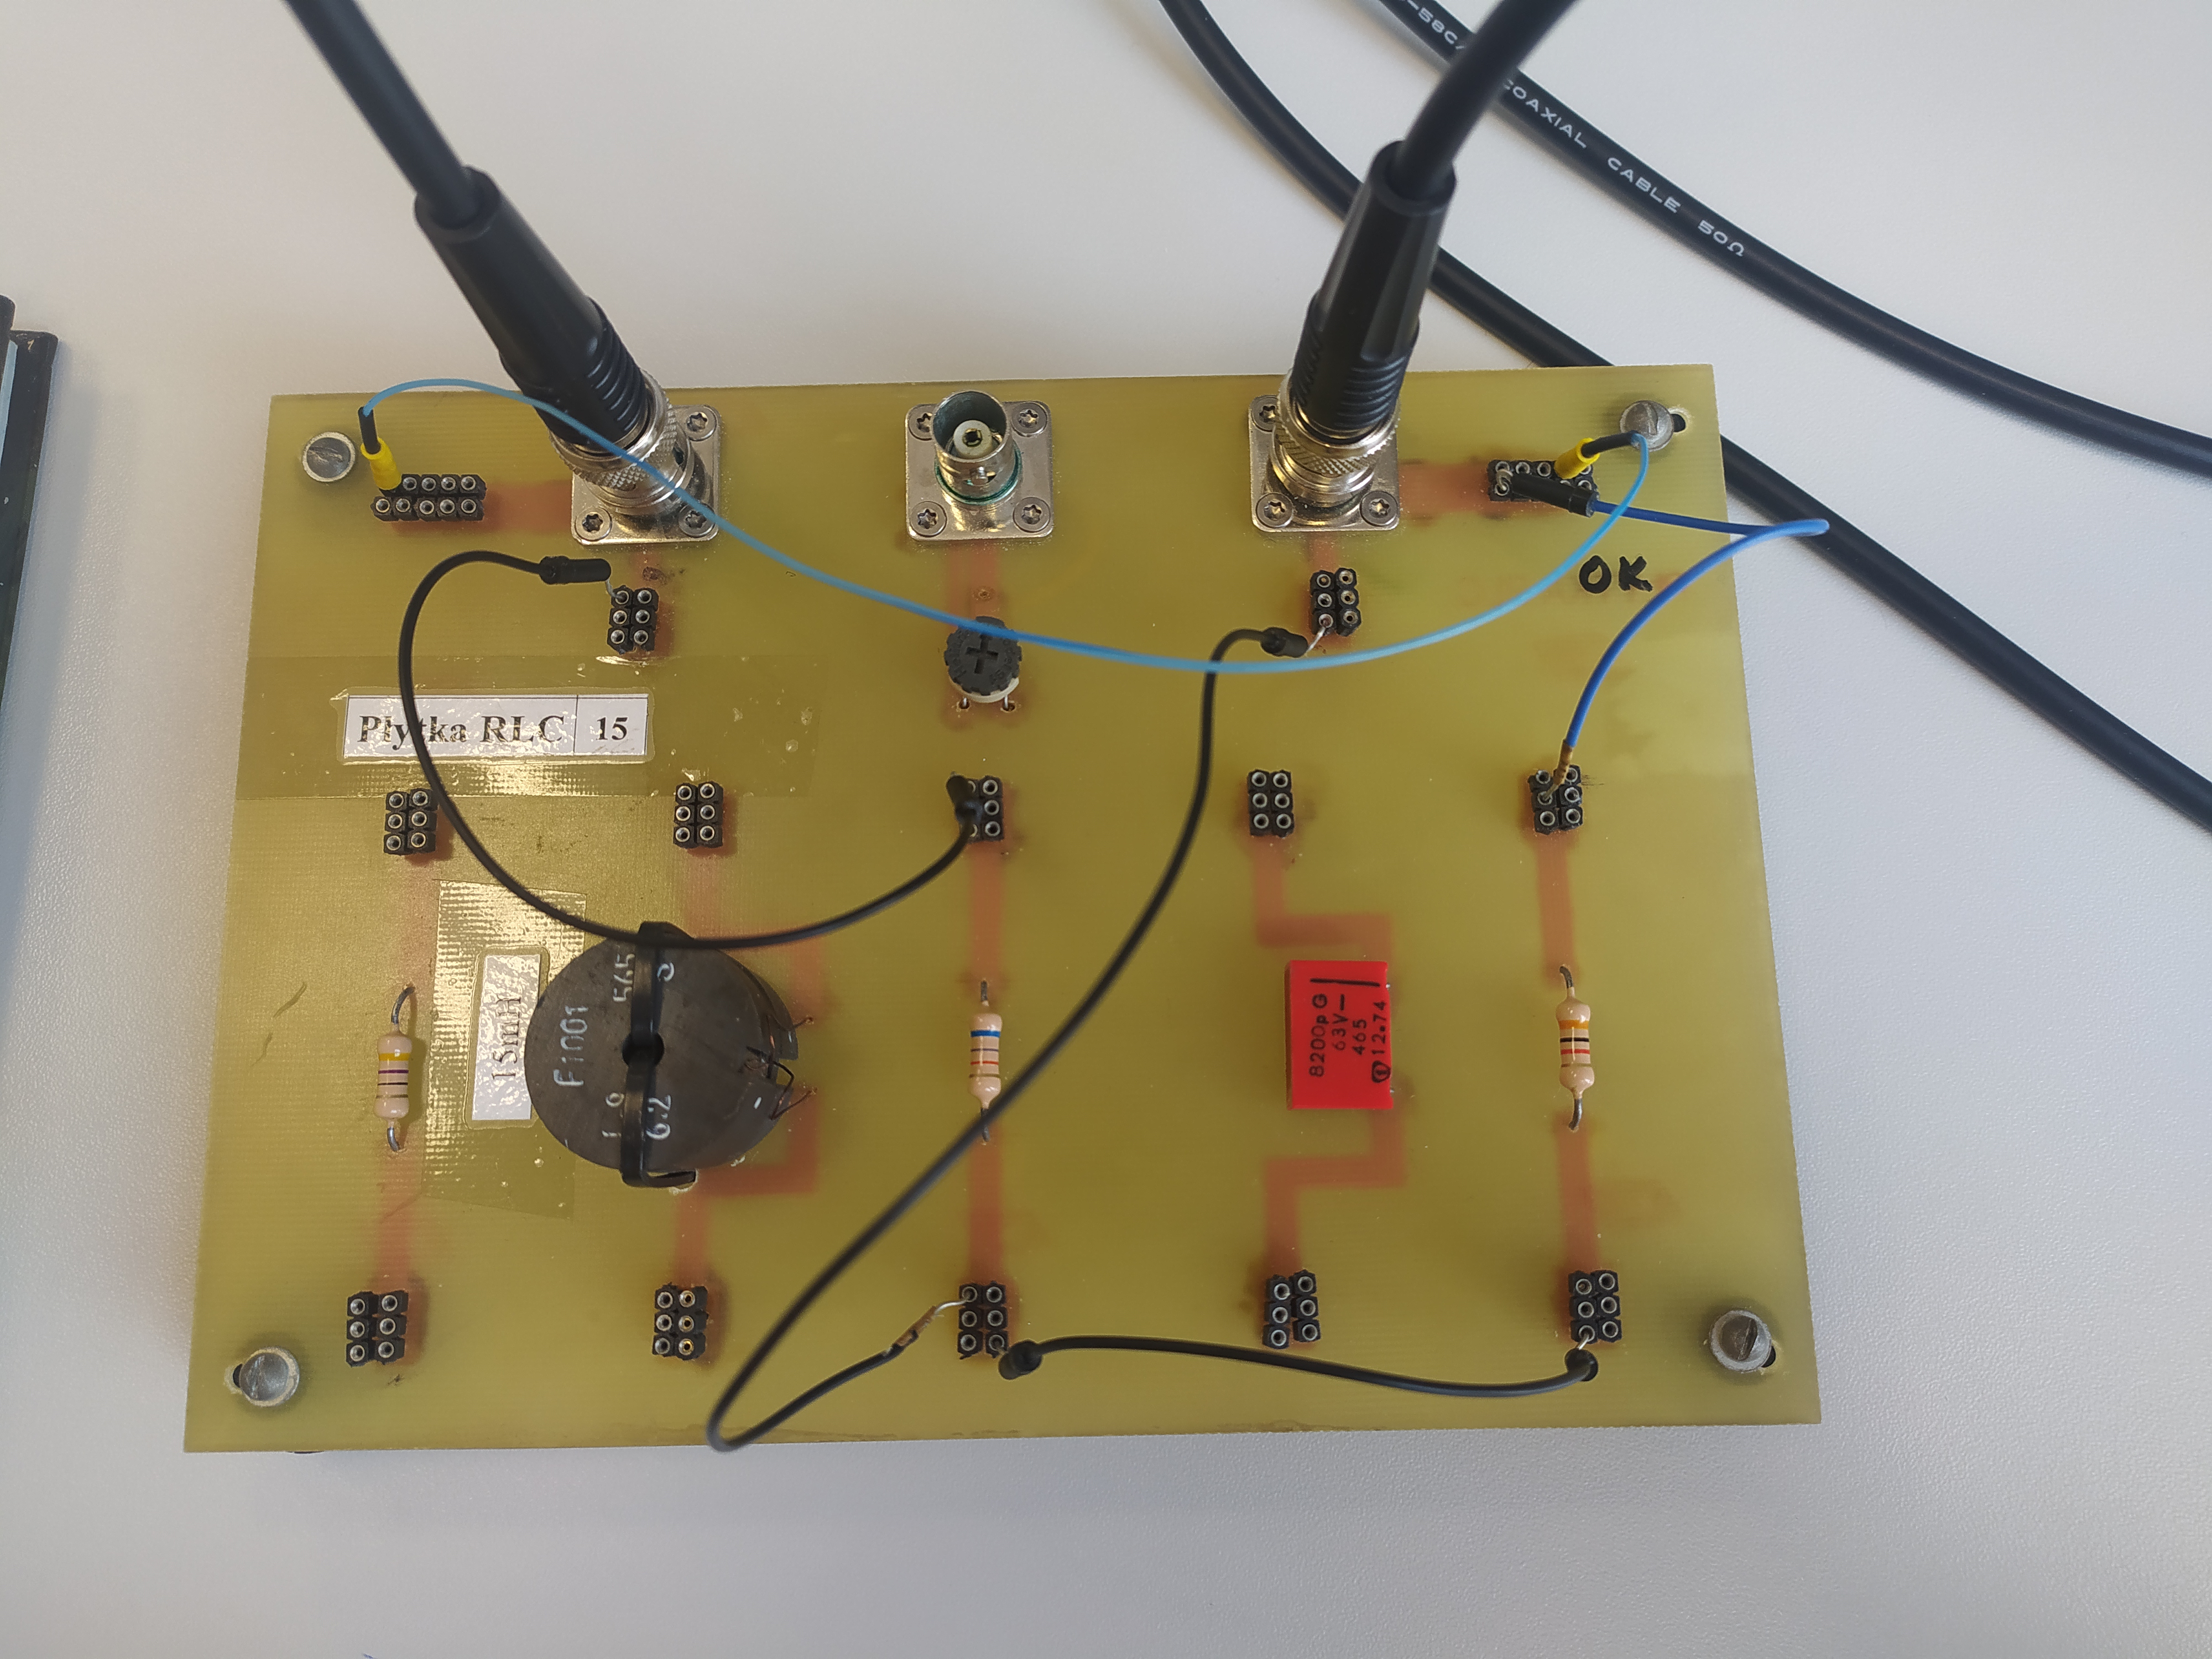
\includegraphics[scale = 0.05]{images/IMG_20220316_113538.jpg}
        \caption{Zbudowany dzielnik}
        \label{fig:my_label}
    \end{figure}
    
\end{itemize}

\section{Pomiary}
    
\begin{itemize}
    \item Teoretyczna wartość $U_{wy}$ wynosi:
    \begin{gather} \label{dzielnik_row}
        U_{wy} = U_{we} \cdot \frac{R_2}{R_1 + R_2} \\\\
        a_t = \frac{R_2}{R_1 + R_2} = \frac{2.987k\Omega}{9.687k\Omega} \approx \textbf{0.308}
    \end{gather}

    Napięcie wyjściowe jest zatem liniowo zależne od napięcia wejściowego.
\end{itemize}
\begin{center}
    \begin{tabular}{|c|c|c|}
         \hline
         $U_{we}$ [V] & Teoretyczna wartość $U_{wy}$ [V] & Zmierzona wartość $U_{wy}$ [V] \\
         \hline
         1 & 0.308 & 0.296\\
         \hline
         2 & 0.616 & 0.616\\
         \hline
         3 & 0.924 & 0.92 \\
         \hline
         4 & 1.232 & 1.22 \\
         \hline
         5 & 1.54  & 1.48 \\
         \hline
         6 & 1.848 & 1.8  \\
         \hline
         7 & 2.156 & 2.08 \\
         \hline
         8 & 2.464 & 2.46 \\
         \hline
         9 & 2.772 & 2.68 \\
         \hline
         10 & 3.08 & 2.96 \\
         \hline
    \end{tabular}
\end{center}



\begin{center}
    \begin{tikzpicture}
        \begin{axis}[
            axis lines = left,
            xlabel = \(U_{we}\),
            x unit = V,
            xtick = {0,1,2,3,4,5,6,7,8,9,10},
            ylabel = {\(U_{wy}\)},
            y unit = V,
            xmin=0, xmax=10,
            ymin=0, ymax=4,
        ]
        \addplot [
            domain=0:10, 
            samples=100, 
            color=red,
        ]
        {0.308 * x};
        \addlegendentry{Teoretyczne wartości}

        \addplot [
            only marks,
            color=blue,
            mark=*,
            ]
            coordinates {
                (1, 0.296)(2,0.616)(3,0.92)(4,1.22)(5,1.48)(6,1.8)(7,2.08)(8,2.46)(9, 2.68)(10, 2.96)
            };
        \addlegendentry{Zmierzone wartości}
        \end{axis}
    \end{tikzpicture}
\end{center}

\pagebreak

\begin{center}
    \textbf{Pomiary dla $U_{we}$ = 1V, 5V, 10V}
\end{center}
\begin{figure}[h]
    \centering
    \includegraphics[scale=0.34]{images/1_7-dzielnik_1V.png}
    \includegraphics[scale=0.34]{images/1_7-dzielnik_5V.png}
    \includegraphics[scale=0.34]{images/1_7-dzielnik_10V.png}
    \label{fig:pomiary_dzielnika}
\end{figure}

\section{Podsumowanie}

\begin{itemize}
    \item Biorąc pod uwagę zmierzone wartości:
    \begin{gather}
       a_z = \frac {\sum^{n} \frac{U_{wy}}{U_{we}}}{n} \\\\
       a_z = \frac{3.01}{10} \\\\
       a_z = \textbf{0.301}
    \end{gather}
    Średni błąd wyniósł:
    \begin{center}
        $|a_t - a_z|$ = \textbf{0.007} \\
    \end{center}
    
    \item Uzyskane pomiary nie różniły się w dużym stopniu od teoretycznych wartości
\end{itemize}

